%%% Local Variables:
%%% mode: latex
%%% TeX-master: "../main_file"
%%% End:

\section{Algorithmes de filtrage basés sur le Time-Table}

La section suivante présente plusieurs algorithmes de filtrage pour le
\CECSP. Tous ces algorithmes utilisant une adaptation du Time-Table
pour le \CUSP, nous commençons donc par présenter ce
raisonnement. Puis, nous présentons deux autres algorithmes permettant
de réduire l'ensemble des valeurs possibles pouvant être prises par
chaque variable. Le premier est adapté du Time-Table disjonctif pour
le \CUSP~\cite{Gay2015} et le dernier utilise une combinaison entre
problème de flots et profil obligatoire.

\subsection{Le Time-Table}
\index{Time-Table!CECSP}
Comme pour le \CUSP, le Time-Table pour le \CECSP~se base sur la
notion de profil obligatoire des activités. Cependant, comme dans le
cas du \CECSP, nous ne connaissons pas la durée exacte d'une activité,
nous utilisons une borne inférieure sur sa durée pour calculer la date
de début au plus tard, $\LS$, et la date de fin au plus tôt,
$\EE$. Pour calculer cette borne, remarquons que la configuration
permettant de finir une activité le plus rapidement possible, est
celle où l'activité est exécutée à son rendement $\bmax$. De ce fait,
une borne inférieure sur la durée de l'activité vaut
$W_i/f_i(\bmax)$. Nous pouvons donc calculer la date de début au plus
tard de l'activité, $\LS=d_i-W_i/f_i(\bmax)$, et sa date de fin au
plus tôt, $\EE=r_i+W_i/f_i(\bmax)$. La partie obligatoire d'une
activité $i$ est alors définie de a même manière que pour le \CUSP:

\begin{defi}
La partie obligatoire d'une activité $i$ est l'intervalle $[\LS,\EE]$.
\end{defi}

Notons que si $\LS \ge \EE$, l'activité $i$ n'a pas de partie
obligatoire. Dans le cas contraire, nous savons que l'activité $i$ va
consommer au moins une quantité $\bmin$ de la ressource durant toute
sa partie obligatoire, et ce, quelque soit le moment où l'activité est
ordonnancée. 


\begin{ex}
Considérons l'activité suivante: 

\vspace{-0.5cm}
\begin{center}
  \begin{tabular}{|P{1cm}P{1cm}P{1cm}P{1cm}P{1cm}P{1cm}|}
    \hline
    \ES & \LE & W_i & \bmin & \bmax & f_i(b)\\
    \hline
    1 & 14 & 72 & 2 & 5 & b+3\\
    \hline
  \end{tabular}
\end{center}

Nous pouvons calculer sa date de début au plus tard,
$\LS=d_i-W_i/f_i(\bmax)=14 - 72/8 =5$, ainsi que sa date de fin au
plus tôt, $\EE=r_i+ W_i/f_i(\bmax)=1 + 72/8 =10$. Comme $\EE > \LS$,
l'activité possède une partie obligatoire qui est l'intervalle
$[5,10]$ (voir
figure~\ref{fig_mand_CECSP_a},~\ref{fig_mand_CECSP_b}). Cependant,
nous pouvons seulement en déduire que l'activité sera en cours dans
cet intervalle et ,grâce à la borne inférieure sur la quantité de
ressource que peut consommer l'activité durant son exécution, nous
pouvons déduire que, sur l'intervalle $[\LS,\EE]$, l'activité est au
moins exécutée à $\bmin$ (voir figure~\ref{fig_mand_CECSP_c}).
  
\begin{figure}[htb!]
\vspace{-0.8cm}
\subcaptionbox{Ordonnancement au plus tôt\label{fig_mand_CECSP_a}}[0.3\linewidth]{
    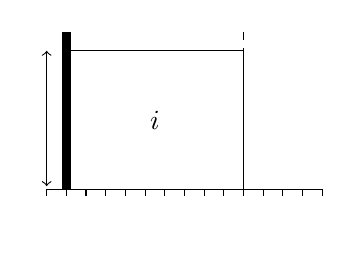
\begin{tikzpicture}
      [xscale=0.25, yscale= 0.4,node distance=0.5cm]
      \node (sil) at (1,0) {} ;
      \node (eil) at (10,0) {} ;
      \node [below of=eil,node distance=0.63cm]  {$\EE$};
      \draw (sil.center) node[below=0.2cm] {$\ES$};
      
      \draw (0,0) -- (14,0);
      \draw[line width=3pt] (1,0) -- (1,5);
      
      \draw[<->] (0,0.1) -- (0,4.4) node[midway,left] {$\bmax$};
      \draw (1,0) rectangle (10,4.4) node[midway] {$i$};

      \draw[dashed] (10,0) -- (10,5);

      \foreach \i in {0,...,14} {
        \draw (\i,0)  -- (\i,-0.2);
      }
    \end{tikzpicture}
}
\hfill
\subcaptionbox{Ordonnancement au plus tard\label{fig_mand_CECSP_b}}[0.3\linewidth]{
    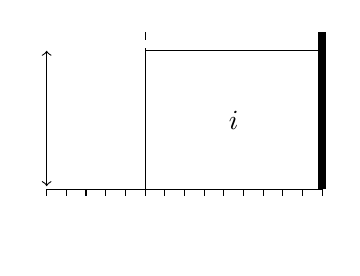
\begin{tikzpicture}
      [xscale=0.25, yscale= 0.4,node distance=0.5cm]
      \node (sir) at (5,0) {} ;
      \node (eir) at (14,0) {} ;
      \node[below of= sir,node distance=0.63cm] {$\LS$};
      \draw (eir.center) node[below=0.2cm] {$\LE$};
      
      \draw (0,0) -- (14,0);
      \draw[line width=3pt] (14,0) -- (14,5);
      
      \draw[<->] (0,0.1) -- (0,4.4) node[midway,left] {$\bmax$};
      \draw (5,0) rectangle (14,4.4) node[midway] {$i$};

      \draw[dashed] (5,0) -- (5,5);

      \foreach \i in {0,...,14} {
        \draw (\i,0)  -- (\i,-0.2);
      }
    \end{tikzpicture}
}
\hfill
\subcaptionbox{Ordonnancement réalisable à $\bmin$ dans
  $[\LS,\EE]$ \label{fig_mand_CECSP_c}}[0.3\linewidth]{ 
    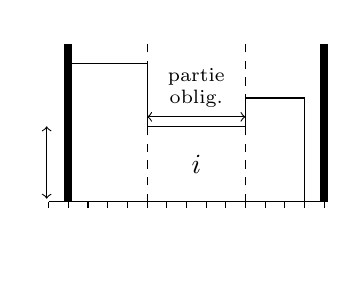
\begin{tikzpicture}
      [xscale=0.25, yscale= 0.4,node distance=0.5cm]
      \node (sir) at (5,0) {} ;
      \node (eil) at (10,0) {} ;
      \node [below of=eil,node distance=0.63cm]  {$\EE$};
      \node[below of= sir,node distance=0.63cm] {$\LS$};
      \draw[<->] (5,2.7) -- (10,2.7) node[midway,above,text width=1.4cm]
      {\begin{center} \scriptsize partie oblig. \end{center}};
      
      \draw[white] (5,0) rectangle (10,2.4) node[midway,color=black] {$i$};
           
      \draw (1,4.4) -- (5,4.4) -- (5,2.4) -- (10,2.4) -- (10,3.3) --
      (13,3.3) -- (13,0);
      
      \draw (0,0) -- (14,0);
      \draw[line width=3pt] (1,0) -- (1,5);
      \draw[line width=3pt] (14,0) -- (14,5);
      
      \draw[<->] (-0.1,0.1) -- (-0.1,2.4) node[midway,left] {$\bmin$};
    


      \draw[dashed] (5,0) -- (5,5);
      \draw[dashed] (10,0) -- (10,5);

      \foreach \i in {0,...,14} {
        \draw (\i,0)  -- (\i,-0.2);
      }
    \end{tikzpicture}
}
\caption{Partie obligatoire d'une activité $i$}
\label{fig_mand_CECSP}
\end{figure}
\end{ex}


En suivant le même cheminement que pour le \CUSP, nous utilisons ces
parties obligatoires pour calculer le profil obligatoire de la
ressource. Ce profil obligatoire est défini comme la somme des parties
obligatoires de toutes les activités. 


\begin{defi} Le {\bf profil obligatoire} d'une ressource $TT_{\cal A}$
est définie par la fonction suivante: $TT_{\cal A}(t)=
\sum_{\substack{i \in {\cal A}\\ \overline{s}_i \le t <
\underline{e}_i}} \bmin,\ \forall t \in {\cal T}$.  Le problème
n'admet pas de solution si $\exists t \in {\cal T}\ : \ TT_{\cal A}(t)
> R$.
\end{defi}


\begin{ex}
  \begin{figure}[!htb]
    \centering
    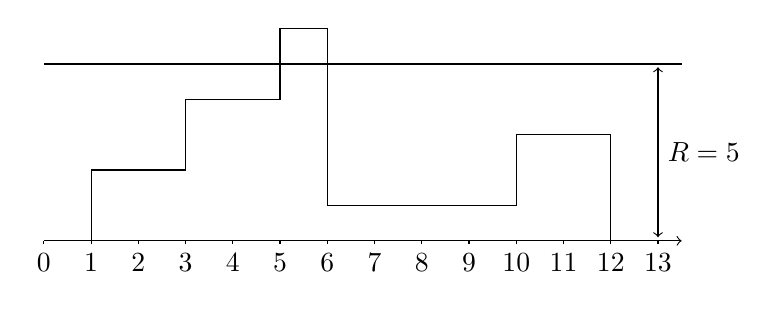
\begin{tikzpicture}
      [yscale=0.45,xscale=0.6]
      \node (O) at (0,0) {};
      \foreach \i in {0,...,13} {
        \draw (\i-1,0) -- (\i-1,-0.1) node[below] {$\i$};
      }
      
      \draw (0,0) -- (0,2) -- (2,2) -- (2,4) -- (4,4) -- (4,6) --
      (5,6) -- (5,1) -- (9,1) -- (9,3) -- (11,3) -- (11,0);
      \draw[->] (-1,0) -- (12.5,0);
      \draw[thick] (-1,5) -- (12.5,5);
      \draw[<->] (12,0.1) -- (12,4.9) node[midway,right] {$R=5$};
    \end{tikzpicture}
    \caption{Exemple de profil obligatoire d'une ressource}
    \label{fig_profil_CECSP}
  \end{figure}
  Dans l'exemple décrit par la figure~\ref{fig_profil_CECSP}, nous
  remarquons que, au temps $t=0$, le profil obligatoire de la
  ressource vaut $2$. Comme la ressource est de capacité $5$, aucune
  incohérence n'est détectée. À l'inverse, au temps $t=4$, le profil
  obligatoire de la ressource a une valeur de $6$, ce qui est
  supérieur à la capacité de la ressource. Une incohérence est donc
  détectée et il n'existe pas de solution réalisable pour cette
  instance. 
\end{ex}


Comme pour le \CUSP, nous pouvons calculer le profil obligatoire d'une
ressource en $O(n)$ à l'aide d'un algorithme de balayage en triant au
préalable les activités par date de début au plus tard et date de fin
au plus tôt (voir algorithme~\ref{algo_profil}).

\begin{algorithm}[!htb]
  \caption{Calcul du profil obligatoire d'une ressource}
  \label{algo_profil}
  $timePoint \gets$ les dates de début/fin au plus tard/tôt
  des activités triées par ordre croissant
  \PourTous {$t \in timePoint$}{
    \Si {$\LS < \EE$}{
      $TT[t]= TT[t-1] +\bmin$}
    \Sinon{
      $TT[t]= TT[t-1]$}
  }
\end{algorithm}

Nous allons maintenant utiliser le raisonnement du Time-Table afin de
définir deux autres algorithmes de filtrage.

\subsection{Le Time-Table disjonctif}

Le second algorithme de filtrage proposé repose sur un raisonnement
appelé Time-Table disjonctif et utilisé, en premier lieu, pour le
\CUSP~\cite{Gay2015}. Comme son nom l'indique, ce dernier repose sur
le raisonnement Time-Table décrit précédemment et sur un raisonnement
appelé raisonnement disjonctif. 

Le raisonnement disjonctif repose sur la construction d'ensembles
disjonctifs. Ces ensembles correspondent aux ensembles d'activités qui
ne peuvent s'exécuter en parallèle. Son application la plus basique
s'intéresse seulement aux ensembles de taille $2$, c'est à dire aux
paires d'activités disjonctives. 

Si nous considérons deux activités $i, j \in \A, i\neq j$ telles que
$\bmin + \bmin[j] > R$ alors une des deux affirmations suivantes doit
être vraie:
\begin{itemize}
\item l'activité $i$ doit commencer après l'activité $j$, ou, 
\item l'activité $i$ doit finir avant l'activité $j$.  
\end{itemize}
En effet, comme les activités $i$ et $j$ ne peuvent être exécutées en
parallèles, l'une doit forcément finir avant que l'autre ne puisse
s'exécuter. 

Cette propriété nous permet d'améliorer les bornes des variables de
début et fin d'une activité. La règle de filtrage est la suivante:

\begin{prop}
Soit $i,j \in \A, i\neq j$ telles que $\bmin + \bmin[j] > R,\ \ES[j] \le
\EE$ et $\LS \le \EE[j]$. Alors la contrainte suivante doit être vérifiée: $et_i\le st_j$. 
\end{prop}

Cette contrainte nous permet, entre autre, d'ajuster la date de début
au plus tôt de $j$. En effet, $\ES[j] \le
\EE$ et $\LS \le \EE[j]$ implique que $j$ doit commencer après la fin
de l'activité $i$ (voir figure~\ref{fig_disj}). De ce fait, la début
de $j$ ne peut arriver avant la date de fin au plus tôt de $i$, et
donc: $\ES[j] \ge \EE$.

\begin{figure}[!htb]
  \centering 
  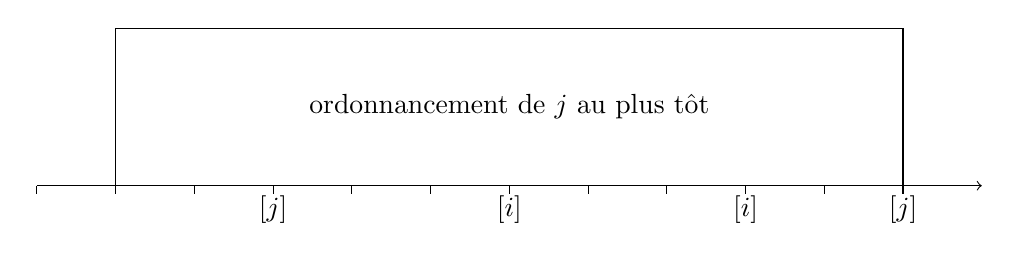
\begin{tikzpicture}
    \node (O) at (0,0) {};
    \draw[->] (0,0) -- (12,0);
    \foreach \i in {0,...,11}
    {\draw (\i,0) -- (\i, -0.1) ;}

    \draw (1,0) node[below] {$\ES$};
    \draw (3,0) node[below] {$\ES[j]$};
    \draw (6,0) node[below] {$\EE[i]$};
    \draw (9,0) node[below] {$\LS[i]$};
    \draw (11,0) node[below] {$\EE[j]$};

    
    \draw (1,0) rectangle (11,2) node[midway] {ordonnancement de $j$
      au plus tôt};
 \end{tikzpicture}
  \caption{Raisonnement disjonctif}
  \label{fig_disj}
\end{figure}

\subsection{Le Time-Table basé sur les flots}


